\subsection{The First Marker}\label{sec:full_marker1}
The first marker, seen in figure \ref{marker:cross}, contains black crossing lines on a white background.
These are two features which can be used to find the marker so both are tested.

Detection using lines was tested, but multiple lines occur in images.
With the used approach it was not possible to reliable detect the marker, so this approach was not considered further.
% so this was not deemed a good method.
The approach is described in appendix \ref{sec:using_lines}.

% \subsubsection{Using Contours}
% The second approach is to use the colors. 
Instead the colors were used.
The marker can be described as a big white rectangle, separated by black lines.
An initial separation of the possible markers is based on the size of the white elements found in the image.
%If the background contains small white blobs, the marker would be bigger.
%If the background is a big white wall, the size of the wall would be larger than the marker so that could be removed based on the size of the object.

The first problem is to find the white elements in an image.
Converting the image to grayscale and selecting threshold the high intensity is an option, but it does not handle shadows and bright areas well.
In figure \ref{fig:threshold_marker1} can the thresholded image be seen and the contours that are detected and within a set size constraint.
The red circle indicates where the marker is found.

\begin{figure}[H]
 \centering
 \begin{subfigure}{\exampleWidth}
 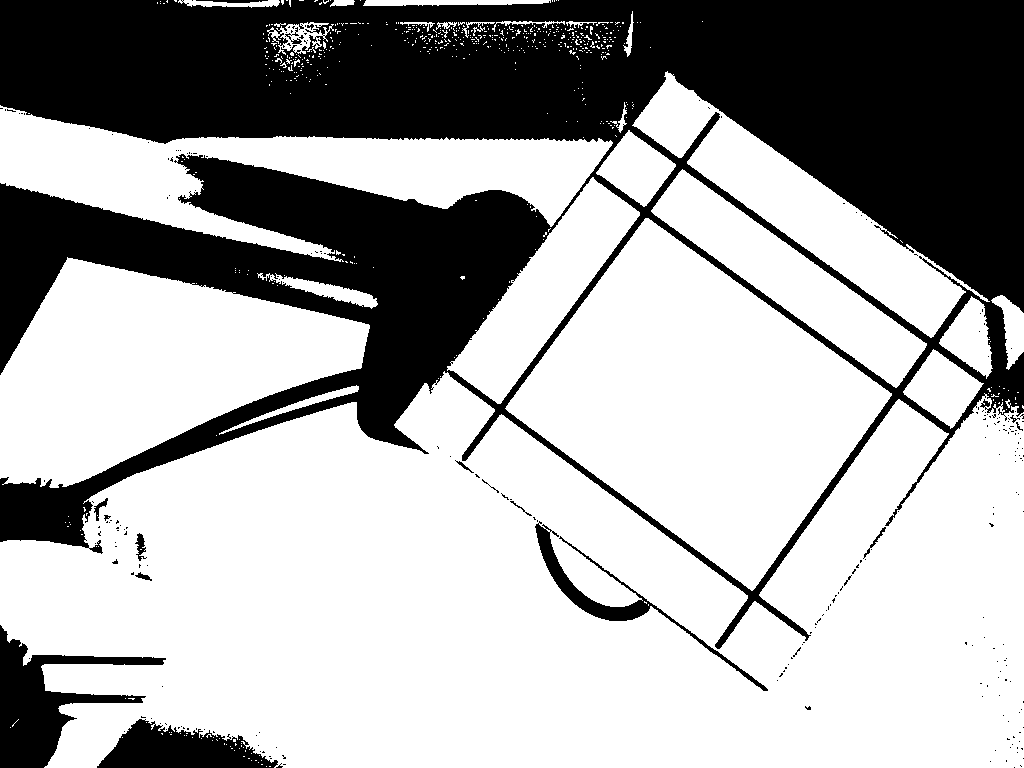
\includegraphics[width=\linewidth]{graphics/threshold_white}
 \caption{White in image.}
 \end{subfigure}
 \begin{subfigure}{\exampleWidth}
 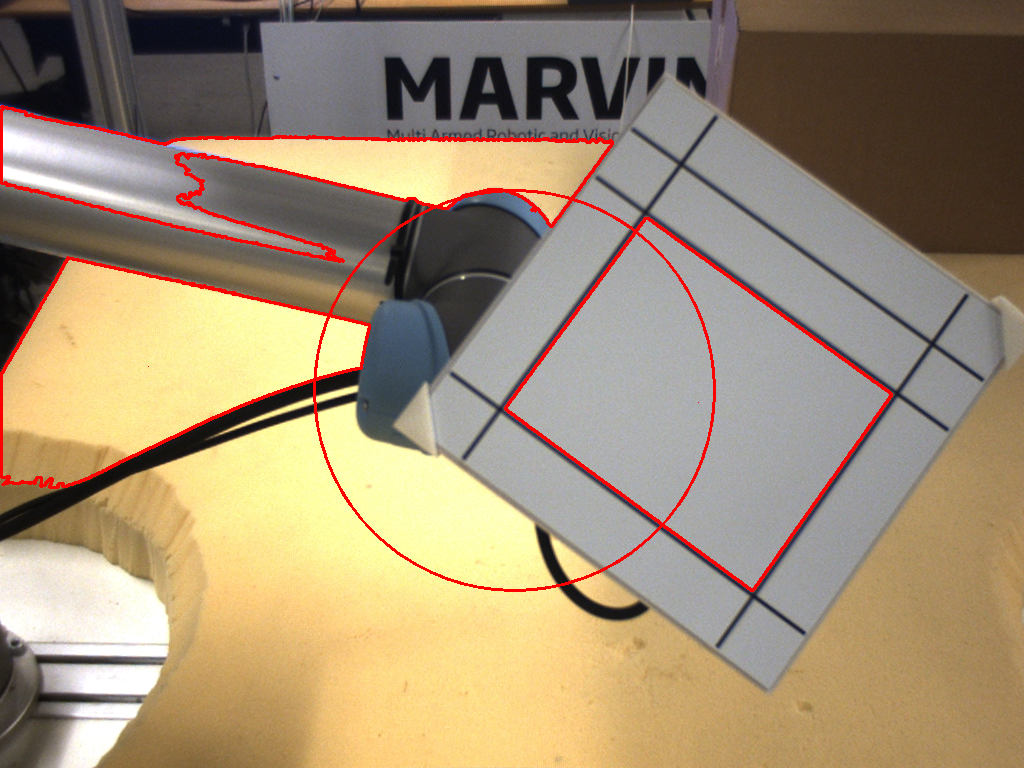
\includegraphics[width=\linewidth]{graphics/threshold_white_contours}
 \caption{Contours detected.}
 \end{subfigure}
 \caption{Detecting the white marker based on grayscale threshold.}
 \label{fig:threshold_marker1}
\end{figure}

%A better way to detect the white part is to split the image into the HSV colorspace.
To get a better result, the image was converted to HSV and perform the same approach as on the grayscale.
To threshold the image for only the white colors, the HSV values with 
%The value is the intensity of the image and selecting the high values gives the same effect as thresholding the grayscale image.
%To remove intense colored parts, the saturation must be set. 
%A low saturation would mean the image is not saturated with a color.
0-20\% saturation and 50-100\% intensity was chosen.
In figure \ref{fig:hsv_intensity} is the intensity shown in relation to the HSV values.

\begin{figure}[H]
\centering
 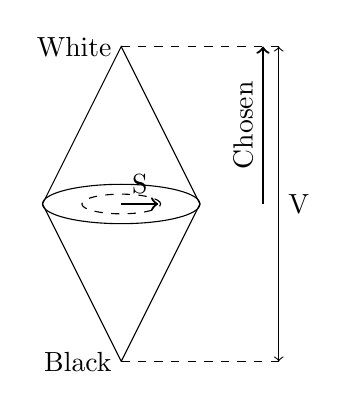
\begin{tikzpicture}
 \draw (0,0) -- (1,2) -- (0,4) -- (-1,2) -- (0,0);
 \draw (0,2) ellipse (1cm and 0.25cm);
 \node[left] at (0,4) {White};
 \node[left] at (0,0) {Black};
 \draw[dashed] (0,2) ellipse (0.5cm and 0.125cm);
 \draw[thick, ->] (0,2) -- ++(0.47,0) node[midway,above,name=s] {S};
 
 \draw[<->] (2,0) -- ++(0,4) node[midway, right] {V};
 \draw[thick, ->] (1.8,2) -- ++(0,2) node[midway, above,rotate=90] {Chosen};
 \draw[dashed] (0,0) -- (2,0) (0,4) -- (2,4);
 \end{tikzpicture}
 \caption[Saturation and intensity in relation to the HSV values.]{Saturation and intensity in relation to the HSV values. Saturation is not to scale in order to illustrate what is taken.}
 \label{fig:hsv_intensity}
\end{figure}


In figure \ref{fig:hsv_marker1} are the white parts and the contours shown for the same area constraints as in figure \ref{fig:threshold_marker1}.
%The HSV values are more robust to changes in the environment and is thus better suited for this assignment.
The HSV values are more reliable at finding true white and is thus better suited for this approach.

\begin{figure}[H]
 \centering
 \begin{subfigure}{\exampleWidth}
 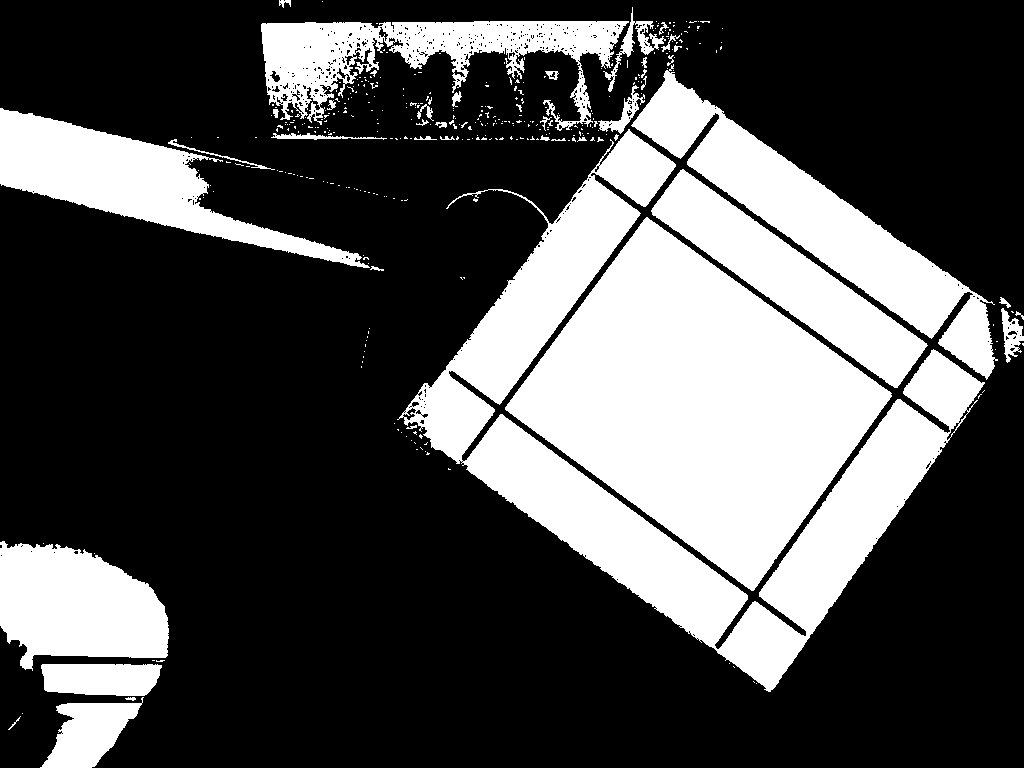
\includegraphics[width=\linewidth]{graphics/hsv_white}
 \caption{White in image.}
 \end{subfigure}
 \begin{subfigure}{\exampleWidth}
 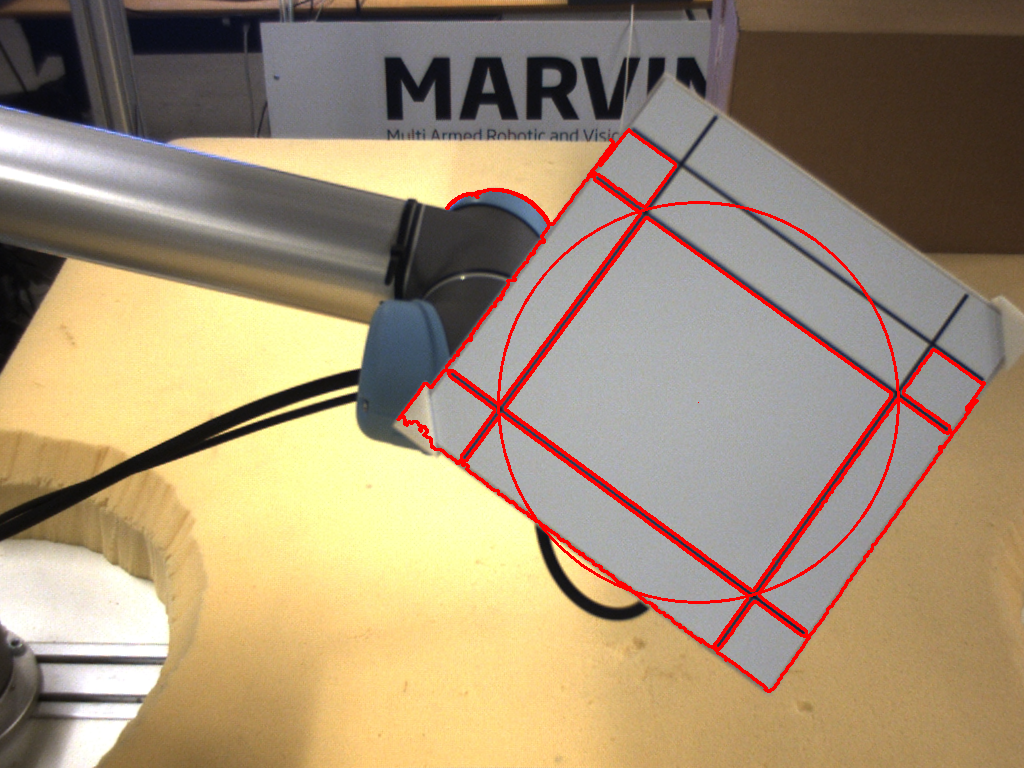
\includegraphics[width=\linewidth]{graphics/hsv_white_contours}
 \caption{Contours detected.}
 \end{subfigure}
 \caption{Detecting the white marker based on HSV threshold.}
 \label{fig:hsv_marker1}
\end{figure}

When the white parts of an image has been detected, the blobs can be found.
%By calculating the areas within the contours, the parts within the size of the marker can be found.
Once found, the center of the marker is found by taking the most compact contour that is closest to the center of the image.
As the robot will be following the position of the marker, this is a good estimate, but it also proved to be good in the images used in the test set as the distracting blobs were not placed in the center, behind the marker.
Using this approach the marker can be found on all the images in the easy and hard set.
To select the appropriate blob as the marker, the both the compactness and the distance to from the center are normalised to a value between zero and one, where one is close to the center and very compact.
The two properties are then scaled and the blob with the highest value is chosen, if it is greater than a minimum threshold.
%\nikolaj{Should I test how many times the marker is found in images where the marker is not there?
%I think it might just always detect the marvin sign or something similar.}

